\documentclass{article}
\usepackage[utf8]{inputenc}
\usepackage{amsmath}
\usepackage{amssymb}
\usepackage{graphicx}
\graphicspath{{.}}

\title{401 HW 1}
\author{James Oswald}
\date{September 2020}

\begin{document}
\maketitle
\addtocounter{section}{2}

\subsection{Continuity, differentiability review}
\paragraph{A)}
Give an example of a function $f:\mathbb{R}\to\mathbb{R}$ that is continuous everywhere on its domain but has at least one point at which it is not differentiable.
\paragraph{}
Using the definition of a continuous function on the real numbers and the definition of a function being differentiable at a point:
\newline\newline
A function $f$ is continuous on the real numbers iff:
\[\forall x\in\mathbb{R}:f(x)\in\mathbb{R}\wedge\lim_{n\to x}f(n) = f(x)\]
Or put more simply, the function is connected with no gaps in its plot. A function $f$ is differentiable at a point x iff:
\[f'(x)\neq DNE := \lim_{h\to 0}\frac{f(p+h) - f(p)}{h}\neq DNE\]
Which basically just states that the derivative of $f$ exists at $x$, or more graphically, the plot of $f$ is "Smooth" at $x$. Using these two definitions, we can easily prove such a function exists just by thinking about the graphs of functions that would satisfy these conditions. We're looking for a connected function with a point where the curve isn't smooth. The first function that comes to mind is $f(x) = |x|$ since thinking about it visually fulfills all the requirements. It is fully connected and therefore continuous, but has no derivative at 0. The proof for continuity is trivial, we know $|x|$ is fully connected since at all points (even 0) the limit of $f$ at $n$  as $n \to x$ is the same as $f(x)$. We can also prove that $|x|$ is not differentiable at $x$ by plugging into the definition. 
\[\lim_{h\to 0}\frac{|0+h| - |0|}{h} = \lim_{h\to 0}\frac{|h|}{h}\]
We see that by splitting this up into the left and right limits, we get it approaching -1 from the left limit and 1 from the right limit, therefore the limit does not exist, and the function is not differentiable at 0.
\newpage
\paragraph{B)}
Give an example of a function $f:\mathbb{R}\to\mathbb{R}$ that is not continuous at 0.
\paragraph{}
Since we're allowed to use a piecewise function, we can easily just define a piecewise function that is explicitly split at 0, for this I will use:
\[f(x) = \begin{cases} 1 & x\leq0 \\0 & x>0 \end{cases}\]
intuitively we know this is discontinuous due to the large gap in its plot, however I will also formalize this by showing it violates the formal definition of continuity of a function at a point provided in part (A). A function $f$ is continuous on the real numbers iff:
\[\forall x\in\mathbb{R}:f(x)\in\mathbb{R}\wedge\lim_{n\to x}f(n) = f(x)\]
We see that at x = 0:
\[\lim_{n\to 0}f(n) = f(0)\]
$f(0) = 1$ but the limit $\lim_{n\to 0}f(n)$ does not exist since approaching from the left yields the limit to be 1 while approaching from the right yields the limit to be 0. Therefore $\lim_{n\to 0}f(n) \neq f(0)$ and the function is not continuous at 0.

\subsubsection{Floating point and related topics}
\paragraph{A)}
Write down the binary expansion of 50.5.
\paragraph{}
I assume this means the IEEE-754 Single Precision floating point expansion. 
\newline
Following the conversion algorithm, I start by converting the whole part, $50$ to binary $110010$. I then convert the decimal portion $.5$ to binary $1$. I then combine them into $110010.1$ which I can then convert to binary scientific notation $1.100101 \cdot 2^5$ The exponent for a single precision float will be the exponent from the sci notation plus 127 so, $5 + 127 = 132$ which in binary will be $10000100$. Our mantissa will be the bits after the decimal from our scientific notation form $100101$, padded by 0s at the end. Finally we put it all together, 1 sign bit, positive in this case (so 0), followed by 8 bits of exponent and the 23 mantissa bits. Using + here to represent concatenation the I get a final answer of:
\[0 + 10000100 + 10010100000000000000000 = 01000010010010100000000000000000\]


\paragraph{B)}
Consider the gaps between representable floating point numbers. Which of the following has the larger gap between it and the next larger representable floating point number? 2 or 201

It should be obvious from the way floating points are stored that 201 has a larger gap than 2 between the next floating point number, since as you gain exponent you loose room for precision in the mantissa which ties in with the fun fact that half of all representable floating point numbers are in the range [-1, 1] and you get less and less precise the further you go out. Just to prove this, I've brute forced the calculations: 

Converting 2 to a float, we get $01000000000000000000000000000000$, the next largest representable float will be $01000000000000000000000000000001$ which is $2.0000002384185791015625$ in decimal. Converting 201 to a 32 bit IEEE 754 float we get $01000011010010010000000000000000$, the next largest representable float will be $01000011010010010000000000000001$ which is $201.0000152587890625$ in decimal. Comparing the distances we get $.0000002384185791015625$ $<\\$ $.0000152587890625$ which proves 201 has a larger gap between it and the next representable number. 

\subsection{Bisection search}
See attached matlab file hw223.m for implementation.
\newline
Code for all 3 parts:
\newline
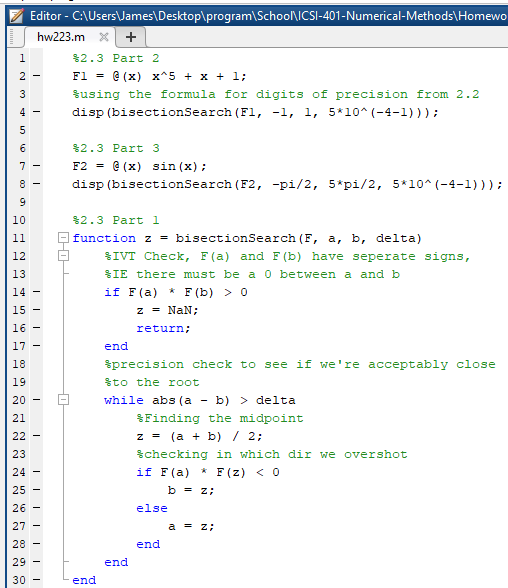
\includegraphics[scale=0.7]{Homework2/2.3code.png}
\newpage
Output For part 2 and 3:
\newline
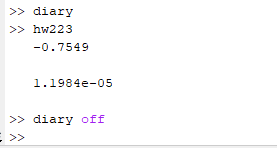
\includegraphics{Homework2/2.3diary.png}
\newline

For part 2, We graph F1 to see that it indeed find the correct root. 
For part 3, we see it found the root at 0, but was stopped by my selection of delta before getting too close.

\subsection{Newton’s method}
See attached matlab file hw224.m file for implementation 

\end{document}